\chapter{Risultati}
In questo capitolo vengono analizzati i risultati ottenuti dall’esecuzione della pipeline. L'impiego di casi rappresentativi facilita la comprensione dei fenomeni alla base del successo o del fallimento delle segmentazioni.

\section{Analisi delle Metriche}
Al fine di analizzare le metriche medie aggregate sull’intero dataset, si considerano i valori riportati nel file \textit{global.csv}, presentati nella Tabella~\ref{tab:global_metrics}.

\begin{table}[H]
\centering
\caption{Metriche medie aggregate sull’intero dataset per le cinque configurazioni sperimentali analizzate.}
\label{tab:global_metrics}
\begin{tabular}{lccc}
\hline
\textbf{Sequenza} & \textbf{Dice Score medio} & \textbf{Sensitivity media} & \textbf{Precision media} \\
\hline
FLAIR & 0.795 & 0.765 & 0.900 \\
T1c & 0.195 & 0.178 & 0.886 \\
T2 & 0.520 & 0.428 & 0.893 \\
Fusion2 & 0.755 & 0.767 & 0.842 \\
Fusion3 & 0.806 & 0.744 & 0.935 \\
\hline
\end{tabular}
\end{table}

È possibile notare come la configurazione \textit{Fusion3} (\textit{FLAIR}+T1c+\textit{T2}) ottenga le migliori prestazioni complessive, con valori medi pari a \textit{Dice Score} \(= 0.806\), \textit{Sensitivity} \(= 0.744\) e \textit{Precision} \(= 0.935\).
La seconda configurazione più efficace risulta essere \textit{FLAIR}, con Dice medio pari a \(0.795\), seguita da \textit{Fusion2} con Dice medio pari a \(0.755\). La sequenza \textit{T2}, invece, presenta prestazioni inferiori con Dice medio pari a \(0.520\), mentre la \textit{T1c} è la configurazione meno affidabile in singolo, con Dice medio pari a \(0.195\).

Nel complesso, i risultati confermano che la fusione multimodale, e in particolare quella trimodale adottata in \textit{Fusion3}, rappresenta la soluzione migliore tra quelle analizzate.

\section{Analisi dei Casi Rappresentativi}
Sono stati selezionati alcuni casi studio a partire dal file \textit{detailed.csv}, individuando i due dei migliori casi e due dei peggiori casi in termini di \textit{Dice Score} sulla configurazione \textit{Fusion3}, come presentato in Tabella~\ref{tab:case_study_dice}.

\begin{table}[H]
\centering
\caption{Valori di \textit{Dice Score} ottenuti nei casi rappresentativi individuati per le cinque configurazioni sperimentali.}
\label{tab:case_study_dice}
\begin{tabular}{lccccc}
\hline
\textbf{Paziente} & \textbf{FLAIR} & \textbf{T1c} & \textbf{T2} & \textbf{Fusion2} & \textbf{Fusion3} \\
\hline
BRATS\_128.nii.gz & 0.879 & 0.048 & 0.645 & 0.318 & 0.963 \\
BRATS\_248.nii.gz & 0.974 & 0.534 & 0.396 & 0.967 & 0.963 \\
BRATS\_140.nii.gz & 0.271 & 0.000 & 0.002 & 0.680 & 0.000 \\
BRATS\_380.nii.gz & 0.000 & 0.000 & 0.000 & 0.000 & 0.000 \\
\hline
\end{tabular}
\end{table}

\subsection{Casi Migliori}

\paragraph{BRATS\_128.nii.gz}
Rappresenta uno dei migliori risultati ottenuti dalla pipeline, con \textit{Dice Score} pari a \(0.963\) sulla configurazione \textit{Fusion3}.

\begin{figure}[H]
    \centering
    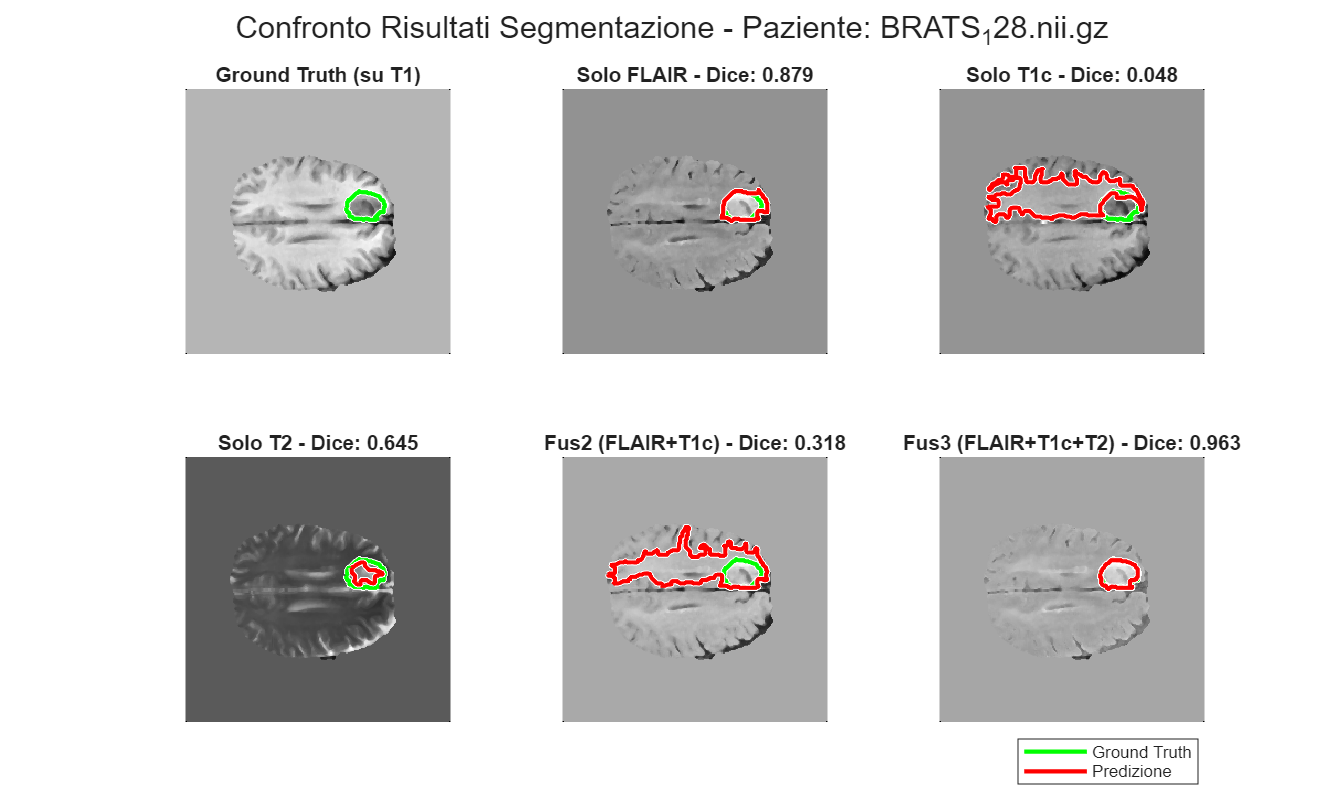
\includegraphics[width=\textwidth]{images/128_comparison_results.png}
    \caption{Confronto finale dei risultati di segmentazione per il paziente 128.}
    \label{fig:res_128}
\end{figure}

Dalla Figura~\ref{fig:res_128} si osserva che la segmentazione ottenuta con \textit{Fusion3} presenta una sovrapposizione quasi completa con la ground truth, seguendo con buona precisione la forma della lesione.

Inizialmente, la lesione appare distinta dal tessuto circostante nella rappresentazione multimodale, facilitando la fase iniziale di sogliatura con Otsu. In questo caso, la combinazione tra \textit{FLAIR} e \textit{T2} valorizza l’estensione della lesione, mentre il contributo ambiguo della \textit{T1c} viene attenuato dalla presenza delle altre modalità. Di conseguenza, la maschera generata su \textit{Fusion3} risulta più vicina alla reale distribuzione del tumore rispetto a \textit{Fusion2}.

Inoltre, la seed map costruita sulla fusione multimodale localizza il seme in una regione interna alla lesione. Questo rende più efficace il Region Growing, che può espandersi in una zona coerente dal punto di vista dell’intensità e della continuità spaziale. Il \textit{Marker-Controlled Watershed} riesce, quindi, a rifinire il contorno senza alterazioni.

Anche la sola sequenza \textit{FLAIR} fornisce un buon risultato, con Dice pari a \(0.879\), mentre la \textit{T2} raggiunge una prestazione intermedia (\(0.645\)). Al contrario, la \textit{T1c} risulta inadeguata, con Dice pari a \(0.048\), poiché produce una segmentazione estesa lungo una fascia orizzontale dell’immagine. Anche \textit{Fusion2} risente di questo comportamento anomalo della \textit{T1c} e ottiene un Dice molto basso (\(0.318\)).

\paragraph{BRATS\_248.nii.gz}
Mostra una prestazione eccellente, con \textit{Dice Score} pari a \(0.963\) sulla configurazione \textit{Fusion3}.

\begin{figure}[H]
    \centering
    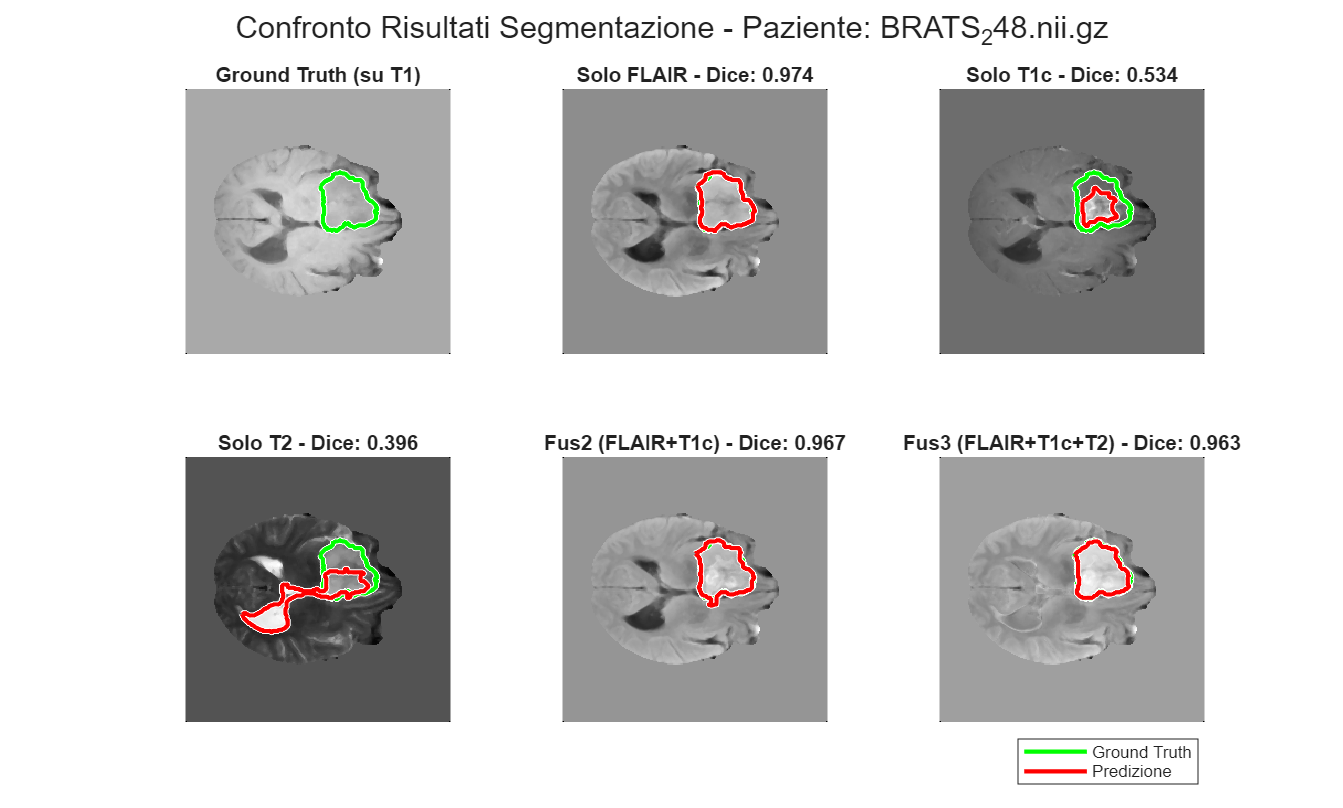
\includegraphics[width=\textwidth]{images/248_comparison_results.png}
    \caption{Confronto finale dei risultati di segmentazione per il paziente 248.}
    \label{fig:res_248}
\end{figure}

Come evidenziato in Figura~\ref{fig:res_248}, la lesione presenta una forma compatta e distinguibile dalle zone circostanti. In tal caso \textit{FLAIR}, \textit{Fusion2} e \textit{Fusion3} riescono a produrre buone segmentazioni. La \textit{FLAIR} raggiunge un Dice pari a \(0.974\), superiore anche alla fusione trimodale, mentre \textit{Fusion2} ottiene \(0.967\) e \textit{Fusion3} \(0.963\).

Il motivo di queste prestazioni elevate risiede nel fatto che, nel paziente considerato, la lesione è ben rappresentata nella sequenza \textit{FLAIR} e, dunque, la sogliatura con Otsu riesce a individuare una regione iniziale già molto vicina alla ground truth. Il \textit{Region Growing} si sviluppa, dunque, attorno a un seme ottimale e il \textit{Marker-Controlled Watershed} beneficia dei contorni regolari e continui del tumore.

Le modalità \textit{T1c} e \textit{T2}, se considerate singolarmente, risultano meno efficaci. La \textit{T1c} produce una segmentazione più contenuta rispetto alla ground truth, mentre la \textit{T2} introduce regioni non coerenti con l'estensione reale della lesione. Tuttavia, quando le informazioni vengono combinate nella fusione multimodale, non compromettono il risultato complessivo.

\subsection{Casi Peggiori}

\paragraph{BRATS\_140.nii.gz}
Rappresenta uno degli esempi più critici della pipeline, con \textit{Dice Score} pari a \(0.000\) sulla configurazione \textit{Fusion3}.

\begin{figure}[H]
    \centering
    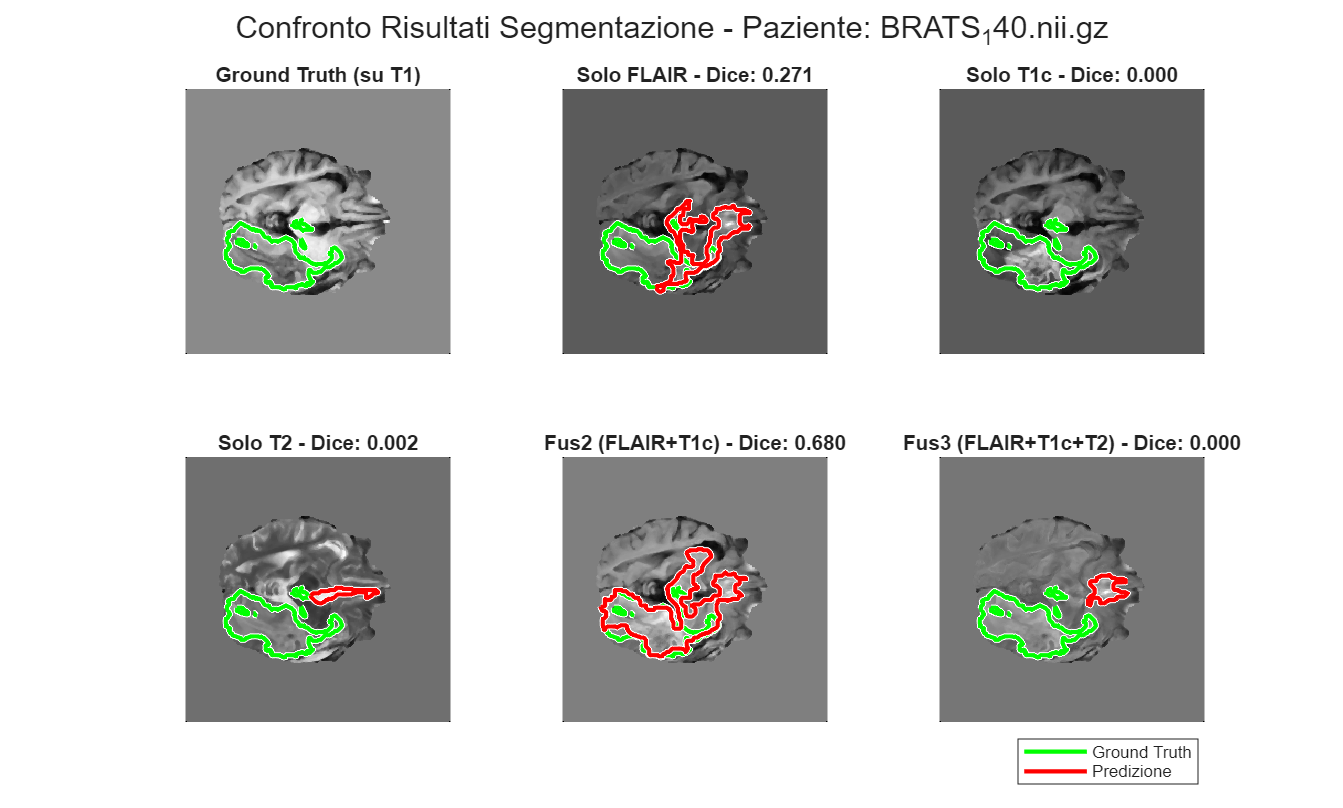
\includegraphics[width=\textwidth]{images/140_comparison_results.png}
    \caption{Confronto finale dei risultati di segmentazione per il paziente 140.}
    \label{fig:res_140}
\end{figure}

Dalla Figura~\ref{fig:res_140} si osserva che la ground truth occupa una regione ampia e irregolare a sinistra dell’immagine, mentre la segmentazione ottenuta con \textit{Fusion3} viene localizzata in una zona spostata verso destra. Di conseguenza, non si verifica alcuna sovrapposizione tra predizione e riferimento e il \textit{Dice Score} risulta nullo.

La \textit{Fusion3} genera una distribuzione di intensità che non valorizza la lesione reale, ma una regione differente dell’immagine. Ciò influisce sulla fase di sogliatura con Otsu, che produce una maschera preliminare non coerente con la posizione del tumore. Di conseguenza, anche la seed map tende a individuare un seme iniziale in una zona non pertinente.

Selezionando un seme errato, l’intera fase di \textit{Region Growing} si sviluppa attorno a una regione sbagliata. Il \textit{Marker-Controlled Watershed} non è in grado di correggere un errore di localizzazione così marcato, poiché lavora sulla maschera preliminare costruita nelle fasi precedenti. Il post-processing morfologico può soltanto regolarizzare la maschera prodotta, ma non recuperarne la posizione corretta.

Anche le altre modalità mostrano un comportamento problematico. La \textit{T1c} fallisce completamente, mentre la \textit{T2} individua una piccola regione errata. La \textit{FLAIR} riesce a intercettare parzialmente la lesione, ma con una segmentazione frammentata. È interessante notare che \textit{Fusion2} ottiene, invece, un risultato poco migliore (\(0.680\)), in quanto l’aggiunta della \textit{T2} nella fusione multimodale introduce un’informazione ambigua che altera la localizzazione corretta della regione tumorale.

\paragraph{BRATS\_380.nii.gz}
Un ulteriore caso di fallimento completo è rappresentato dal paziente \textit{BRATS\_380.nii.gz}, per il quale tutte le configurazioni principali mostrano \textit{Dice Score} pari a \(0.000\).

\begin{figure}[H]
    \centering
    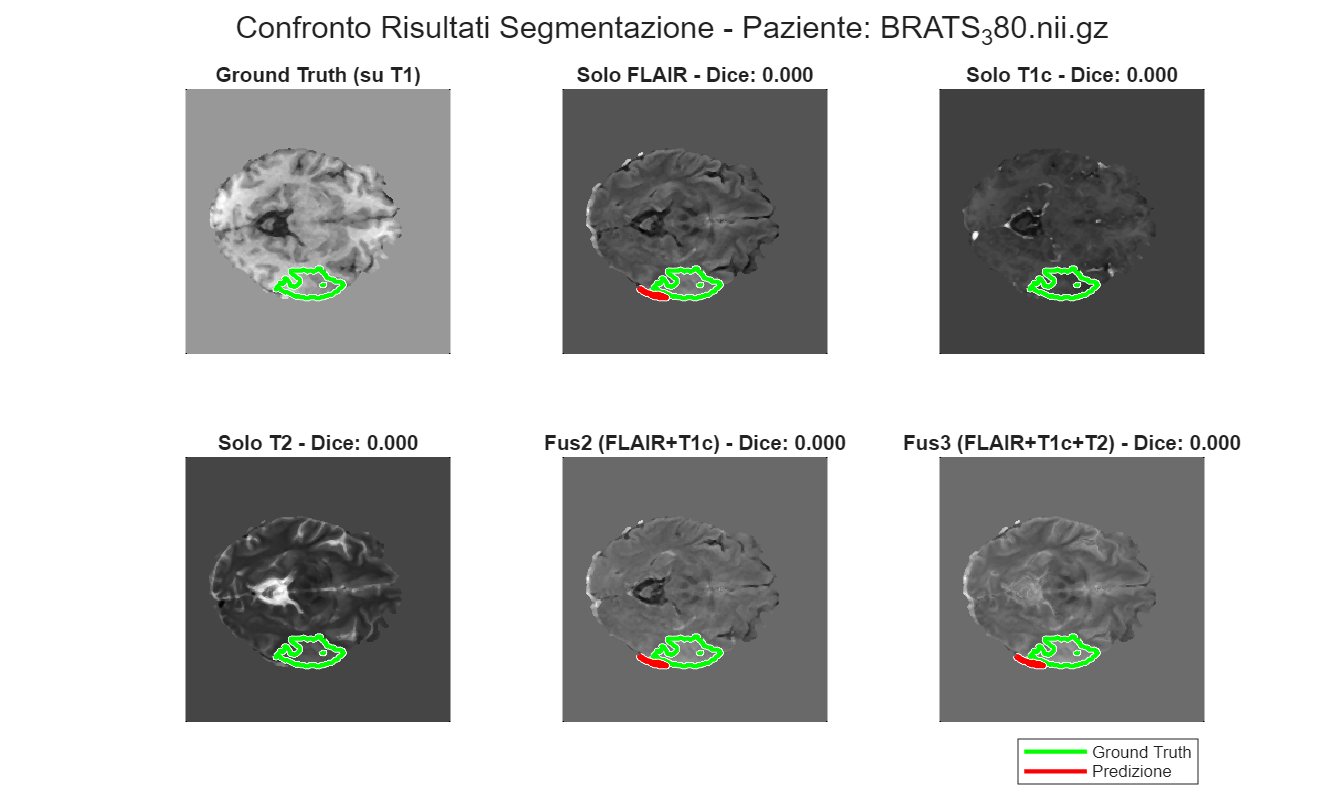
\includegraphics[width=\textwidth]{images/380_comparison_results.png}
    \caption{Confronto finale dei risultati di segmentazione per il paziente 380.}
    \label{fig:res_380}
\end{figure}

Come mostrato in Figura~\ref{fig:res_380}, la ground truth è posizionata in una piccola regione nella parte inferiore dell’immagine, mentre le predizioni prodotte dalla pipeline risultano assenti oppure collocate lateralmente. In nessun caso si realizza una sovrapposizione sufficiente con la ground truth.

Il fallimento è dovuto alle caratteristiche intrinseche della lesione, che appare piccola e poco evidente rispetto al contesto circostante. Una configurazione di questo tipo rende complicata la fase di sogliatura iniziale, poiché il tumore e il tessuto sano non presentano livelli di intensità nettamente separabili nell'istogramma. Inoltre, anche la generazione della seed map diventa meno affidabile, dato che la sfocatura gaussiana privilegia aree a intensità più marcata che non coincidono con una lesione piccola e poco contrastata.